\begin{frame}
	\frametitle{Custo M\'edio e Lucro}
	Em geral:
	\begin{align*}
		\text{Lucro} &= \text{Receita Total} - \text{Custo Total}\\
		\Pi &= RT - CT \\
		\Pi &= PQ-CF-CV \\
		\Pi &= Q(P-CTM) = Q(P-CVM-CFM)
	\end{align*}

	Se o pre\c co unit\'ario de venda do bem for suficientemente grande, $P>CTM$, a empresa ter\'a lucro, caso contr\'ario, ter\'a prejuizo.
\end{frame}

\begin{frame}
	\frametitle{Custo M\'edio e Lucro}
	\[\Pi=Q(P-CVM-CFM)\]
	Quando h\'a preju\'izo, ele pode ter naturezas muito diferentes:
	\begin{itemize}
		\item $P-CVM>0$, mas inferior a $CFM$: a receita \'e suficiente para pagar os factores vari\'aveis, mas n\~ao chega para a totalidade dos factores fixos, havendo preju\'izo a curto prazo
		\item $P-CVM<0$, a empresa \'e insustent\'avel: as receitas nem sequer cobrem o custo vari\'avel
	\end{itemize}
\end{frame}

\begin{frame}
	\frametitle{Maximiza\c c\~ao do Lucro Econ\'omico; Escolha \'Optima da empresa}
	Cada empresa pretende encontrar a quantidade a produzir tal que: \[Max \Pi = RT-CT\]
	Sendo:\[\Pi=pQ_i-CV(Q_i)-CF\]
	CPO:\ \(\frac{d\Pi}{dQ_i} = 0 \Leftrightarrow p-CV'=0\Leftrightarrow p=CMg\) \\
	CSO:\ \(\frac{d^2\Pi}{dQ_i^2} < 0 \Leftrightarrow -\frac{dCMg}{dQ_i}<0\Leftrightarrow\frac{dCMg}{dQ_i}>0 \Leftrightarrow \text{CMg crescente}\)
\end{frame}

\begin{frame}
	\frametitle{Maximiza\c c\~ao do Lucro}
	A quantidade \'optima a produzir \'e tal que $p=CMg$ na zona ascendente da curva de $CMg$. Dado um pre\c co $P^*$, ent\~ao a quantidade \'optima \'e $Q_i^*$.
	\begin{center}
		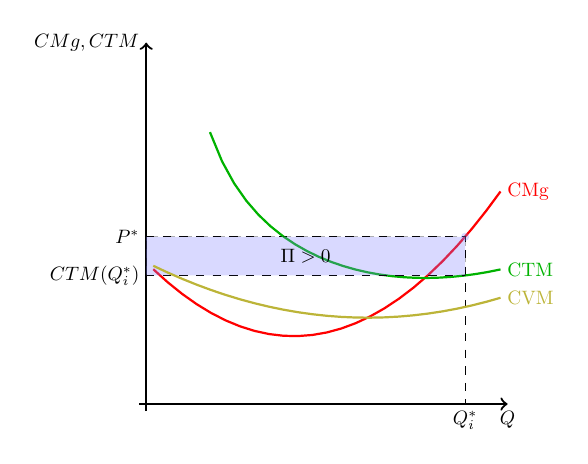
\begin{tikzpicture}[
			scale = 0.9,
			every node/.style = {scale =0.7},
			declare function = {
				cv(\x) = \x - (1/4)*\x^2 + (1/25)*\x^3;
				cf(\x) = 1;
				ct(\x) = cv(\x) + cf(\x);
				cmg(\x) = 1 - (2/4)*\x + (3/25)*\x^2;
				ctm(\x) = ct(\x)/\x;
				cvm(\x) = cv(\x)/\x;
			}
		]

			\def\p{4.5}

			\draw[->,thick] (-0.1,-0) -- (5.1,-0) node[below]{$Q$};
			\draw[->,thick] (0,-0.1) -- (0,5.1) node[left]{$CMg,CTM$};

			\onslide<2->{
				\draw[red,thick,domain=0.1:5,variable=\x] plot (\x,{2*cmg(\x)-0});
				\draw[red](5,{2*cmg(5)-0})node[right]{CMg};
			}
			\onslide<3->{
				\draw[dashed] (0,{2*cmg(\p)})node[left]{$P^*$} -- (\p,{2*cmg(\p)}) -- (\p,0)node[below]{$Q_i^*$};		
			}

			\onslide<4->{
				\draw[green!70!black,thick,domain=0.9:5,variable=\x] plot (\x,{2*ctm(\x)-0});
				\draw[green!70!black](5,{2*ctm(5)-0})node[right]{CTM};
			}

			\onslide<5->{
				\draw[dashed] (0,{2*ctm(\p)})node[left]{$CTM(Q_i^*)$} -- (\p,{2*ctm(\p)});		
			}

			\onslide<6->{
				\draw[dashed,fill=blue!50!white,opacity=0.3] (0,{2*ctm(\p)}) -- (\p,{2*ctm(\p)}) --(\p,{2*cmg(\p)}) node[circle,fill,inner sep = 1.5]{} -- (0,{2*cmg(\p)}) -- (0,{2*ctm(\p)});
				\draw({\p/2},{(2*cmg(\p)+2*ctm(\p))/2}) node{$\Pi>0$};
			}
			
			\onslide<7->{
				\draw[yellow!70!black,thick,domain=0.1:5,variable=\x] plot (\x,{2*cvm(\x)-0});
				\draw[yellow!70!black](5,{2*cvm(5)-0})node[right]{CVM};
			}			

		\end{tikzpicture}
	\end{center}
\end{frame}


\begin{frame}
	\frametitle{Maximiza\c c\~ao do Lucro}
	A quantidade \'optima a produzir \'e tal que $p=CMg$ na zona ascendente da curva de $CMg$. Dado um pre\c co $P^*$, ent\~ao a quantidade \'optima \'e $Q_i^*$ e h\'a um preju\'izo!
	\begin{center}
		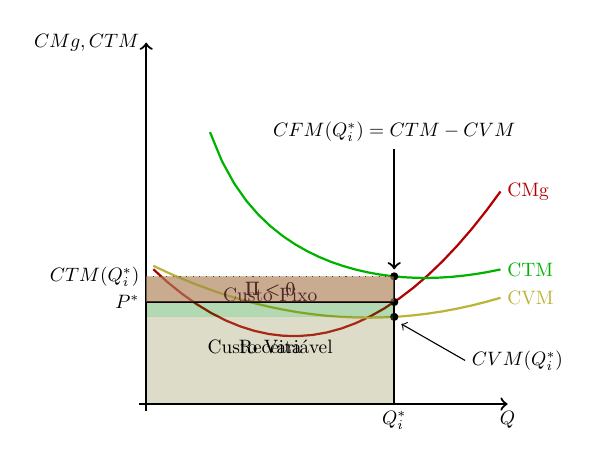
\begin{tikzpicture}[
			scale = 0.9,
			every node/.style = {scale =0.7},
			declare function = {
				cv(\x) = \x - (1/4)*\x^2 + (1/25)*\x^3;
				cf(\x) = 1;
				ct(\x) = cv(\x) + cf(\x);
				cmg(\x) = 1 - (2/4)*\x + (3/25)*\x^2;
				ctm(\x) = ct(\x)/\x;
				cvm(\x) = cv(\x)/\x;
			}
		]

			\def\p{3.5}

			\draw[->,thick] (-0.1,-0) -- (5.1,-0) node[below]{$Q$};
			\draw[->,thick] (0,-0.1) -- (0,5.1) node[left]{$CMg,CTM$};

			
			\draw[red!70!black,thick,domain=0.1:5,variable=\x] plot (\x,{2*cmg(\x)-0});
			\draw[red!70!black](5,{2*cmg(5)-0})node[right]{CMg};	
			

			\onslide<2->{
				\draw[dotted] (0,{2*cmg(\p)})node[left]{$P^*$} -- (\p,{2*cmg(\p)});
			}

			\onslide<3->{
				\draw[dotted] (\p,0)node[below]{$Q_i^*$}--(\p,{2*cmg(\p)})node[circle,fill,inner sep=1.5pt]{};
			}

			\onslide<4->{
				 \draw[green!70!black,thick,domain=0.9:5,variable=\x] plot (\x,{2*ctm(\x)-0});	
				 \draw[green!70!black](5,{2*ctm(5)-0})node[right]{CTM};
				 
				 \draw[dotted] (\p,{2*cmg(\p)}) -- (\p,{2*ctm(\p)})node[circle,fill,inner sep=1.5pt]{};
				 \draw[dotted] (0,{2*ctm(\p)})node[left]{$CTM(Q_i^*)$} -- (\p,{2*ctm(\p)});
			}

			\onslide<5-9>{
				\draw({\p/2},{(2*cmg(\p)+2*ctm(\p))/2}) node{$\Pi<0$};
				\draw[draw=none,fill=red!50!white,opacity=0.3] (0,{2*ctm(\p)}) -- (\p,{2*ctm(\p)}) --(\p,{2*cmg(\p)}) -- (0,{2*cmg(\p)}) -- (0,{2*ctm(\p)});
			}

			\onslide<6->{
				\draw[yellow!70!black,thick,domain=0.1:5,variable=\x] plot (\x,{2*cvm(\x)-0});
				\draw[yellow!70!black](5,{2*cvm(5)-0})node[right]{CVM};
			}

			\onslide<7->{
				\draw[<-] (\p+0.1,{2*cvm(\p)-0.1}) -- ({\p+1},{cvm(\p)}) node[right]{$CVM(Q_i^*)$};
				\draw[] (\p,{2*cvm(\p)}) node[circle,fill,inner sep=1.5pt]{};
			}

			\onslide<8->{
				\draw[<-,thick] ({\p},{2*ctm(\p)+0.1}) -- ({\p},{4*ctm(\p)})node[above]{$CFM(Q_i^*)=CTM-CVM$};
				\draw[thick] (\p,{2*cvm(\p)}) -- (\p,{2*ctm(\p)});
			}

			\onslide<9->{
				\draw[thick,red] (\p,{2*cvm(\p)}) -- (\p,{2*cmg(\p)});	
			}

			\onslide<10-11>{
				\draw[draw=none,fill=green!50!black,opacity=0.3] (0,{2*ctm(\p)}) -- (\p,{2*ctm(\p)}) --(\p,{2*cvm(\p)}) -- (0,{2*cvm(\p)}) -- (0,{2*ctm(\p)});

				\draw[draw=none,fill=yellow!50!black,opacity=0.3] (0,{2*cvm(\p)}) -- (\p,{2*cvm(\p)}) --(\p,0) -- (0,0) -- (0,{2*cvm(\p)});
			}

			\onslide<10>{
				\draw({\p/2},{(2*cmg(\p)+2*ctm(\p))/2.1}) node{Custo Fixo};
				\draw({\p/2},{(2*cmg(\p)+2*ctm(\p))/4}) node{Custo Vari\'avel};
			}

			\onslide<11>{
				\draw[thick] (0,0) -- (\p,0) -- (\p,{2*cmg(\p)}) -- (0,{2*cmg(\p)}) -- (0,0);
				\draw({\p/2},{(2*cmg(\p)+2*ctm(\p))/4}) node{Receita};
			}

			\onslide<12>{
				\draw({\p/2},{(2*cmg(\p)+2*ctm(\p))/2}) node{$\Pi<0$};
				\draw[draw=none,fill=red!50!white,opacity=0.3] (0,{2*ctm(\p)}) -- (\p,{2*ctm(\p)}) --(\p,{2*cmg(\p)}) -- (0,{2*cmg(\p)}) -- (0,{2*ctm(\p)});
			}

		\end{tikzpicture}
	\end{center}
\end{frame}


\begin{frame}
	\frametitle{Maximiza\c c\~ao do Lucro}
	A quantidade \'optima a produzir \'e tal que $p=CMg$ na zona ascendente da curva de $CMg$. Dado um pre\c co $P^*$, ent\~ao a quantidade \'optima \'e $Q_i^*$ e h\'a um preju\'izo superior a $CF$!
	\begin{center}
		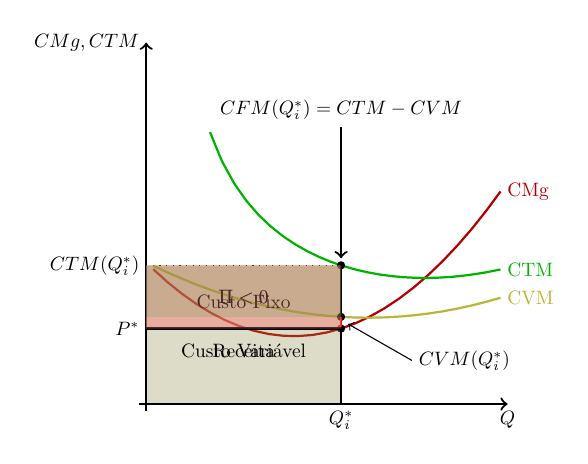
\begin{tikzpicture}[
			scale = 0.9,
			every node/.style = {scale =0.7},
			declare function = {
				cv(\x) = \x - (1/4)*\x^2 + (1/25)*\x^3;
				cf(\x) = 1;
				ct(\x) = cv(\x) + cf(\x);
				cmg(\x) = 1 - (2/4)*\x + (3/25)*\x^2;
				ctm(\x) = ct(\x)/\x;
				cvm(\x) = cv(\x)/\x;
			}
		]

			\def\p{2.75}

			\draw[->,thick] (-0.1,-0) -- (5.1,-0) node[below]{$Q$};
			\draw[->,thick] (0,-0.1) -- (0,5.1) node[left]{$CMg,CTM$};

			
			\draw[red!70!black,thick,domain=0.1:5,variable=\x] plot (\x,{2*cmg(\x)-0});
			\draw[red!70!black](5,{2*cmg(5)-0})node[right]{CMg};	
			

			\onslide<2->{
				\draw[dotted] (0,{2*cmg(\p)})node[left]{$P^*$} -- (\p,{2*cmg(\p)});
			}

			\onslide<3->{
				\draw[dotted] (\p,0)node[below]{$Q_i^*$}--(\p,{2*cmg(\p)})node[circle,fill,inner sep=1.5pt]{};
			}

			\onslide<4->{
				 \draw[green!70!black,thick,domain=0.9:5,variable=\x] plot (\x,{2*ctm(\x)-0});	
				 \draw[green!70!black](5,{2*ctm(5)-0})node[right]{CTM};
				 
				 \draw[dotted] (\p,{2*cmg(\p)}) -- (\p,{2*ctm(\p)})node[circle,fill,inner sep=1.5pt]{};
				 \draw[dotted] (0,{2*ctm(\p)})node[left]{$CTM(Q_i^*)$} -- (\p,{2*ctm(\p)});
			}

			\onslide<5-9>{
				\draw({\p/2},{(2*cmg(\p)+2*ctm(\p))/2}) node{$\Pi<0$};
				\draw[draw=none,fill=red!50!white,opacity=0.3] (0,{2*ctm(\p)}) -- (\p,{2*ctm(\p)}) --(\p,{2*cmg(\p)}) -- (0,{2*cmg(\p)}) -- (0,{2*ctm(\p)});
			}

			\onslide<6->{
				\draw[yellow!70!black,thick,domain=0.1:5,variable=\x] plot (\x,{2*cvm(\x)-0});
				\draw[yellow!70!black](5,{2*cvm(5)-0})node[right]{CVM};
			}

			\onslide<7->{
				\draw[<-] (\p+0.1,{2*cvm(\p)-0.1}) -- ({\p+1},{cvm(\p)}) node[right]{$CVM(Q_i^*)$};
				\draw[] (\p,{2*cvm(\p)}) node[circle,fill,inner sep=1.5pt]{};
			}

			\onslide<8->{
				\draw[<-,thick] ({\p},{2*ctm(\p)+0.1}) -- ({\p},{4*ctm(\p)})node[above]{$CFM(Q_i^*)=CTM-CVM$};
				\draw[thick] (\p,{2*cvm(\p)}) -- (\p,{2*ctm(\p)});
			}

			\onslide<9->{
				\draw[thick,red] (\p,{2*cvm(\p)}) -- (\p,{2*cmg(\p)});	
			}

			\onslide<10-11>{
				\draw[draw=none,fill=green!50!black,opacity=0.3] (0,{2*ctm(\p)}) -- (\p,{2*ctm(\p)}) --(\p,{2*cvm(\p)}) -- (0,{2*cvm(\p)}) -- (0,{2*ctm(\p)});

				\draw[draw=none,fill=yellow!50!black,opacity=0.3] (0,{2*cvm(\p)}) -- (\p,{2*cvm(\p)}) --(\p,0) -- (0,0) -- (0,{2*cvm(\p)});
			}

			\onslide<10>{
				\draw({\p/2},{(2*cmg(\p)+2*ctm(\p))/2.1}) node{Custo Fixo};
				\draw({\p/2},{(2*cmg(\p)+2*ctm(\p))/4}) node{Custo Vari\'avel};
			}

			\onslide<11>{
				\draw[thick] (0,0) -- (\p,0) -- (\p,{2*cmg(\p)}) -- (0,{2*cmg(\p)}) -- (0,0);
				\draw({\p/2},{(2*cmg(\p)+2*ctm(\p))/4}) node{Receita};
			}

			\onslide<12>{
				\draw({\p/2},{(2*cmg(\p)+2*ctm(\p))/2}) node{$\Pi<0$};
				\draw[draw=none,fill=red!50!white,opacity=0.3] (0,{2*ctm(\p)}) -- (\p,{2*ctm(\p)}) --(\p,{2*cmg(\p)}) -- (0,{2*cmg(\p)}) -- (0,{2*ctm(\p)});
			}

		\end{tikzpicture}
	\end{center}
\end{frame}

\begin{frame}
	\frametitle{Lucro ou Preju\'izo?}
	\begin{itemize}
		\setlength{\itemsep}{15pt}
		\item $\Pi^* = P^*Q^*-CTM(Q_i^*)Q_i^* = RT^*-CT^*$
		\item $\Pi^*>0\Leftrightarrow P^*Q_i^*>CTM(Q_i^*)Q_i^*\Leftrightarrow P^*>CTM$
		\item $\Pi^*<0\Leftrightarrow P^* < CTM \Rightarrow$ o preju\'izo \'e inferior a $CF$
		\item $P^*<CMV\Rightarrow\Pi^*<-CF\Rightarrow$ Encerrar!, e ter\'a apenas $CF$ como preju\'izo
	\end{itemize}
\end{frame}


\begin{frame}
	\frametitle{Rendibilidade e Encerramento a curto prazo}

	\begin{center}
		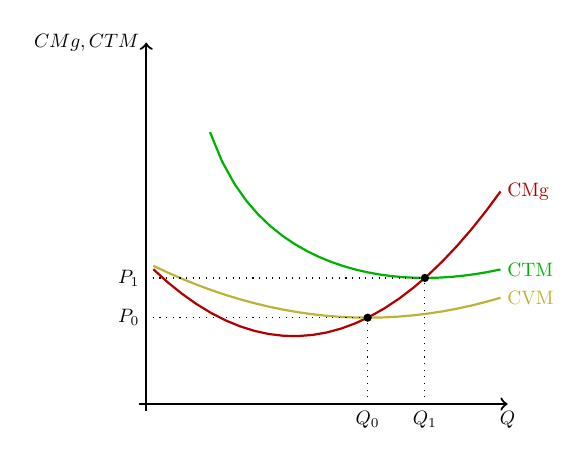
\begin{tikzpicture}[
			scale = 0.9,
			every node/.style = {scale =0.7},
			declare function = {
				cv(\x) = \x - (1/4)*\x^2 + (1/25)*\x^3;
				cf(\x) = 1;
				ct(\x) = cv(\x) + cf(\x);
				cmg(\x) = 1 - (2/4)*\x + (3/25)*\x^2;
				ctm(\x) = ct(\x)/\x;
				cvm(\x) = cv(\x)/\x;
			}
		]

			\def\p{3.9330669}
			\def\q{25/8}

			\draw[->,thick] (-0.1,-0) -- (5.1,-0) node[below]{$Q$};
			\draw[->,thick] (0,-0.1) -- (0,5.1) node[left]{$CMg,CTM$};

			
			\draw[red!70!black,thick,domain=0.1:5,variable=\x] plot (\x,{2*cmg(\x)-0});
			\draw[red!70!black](5,{2*cmg(5)-0})node[right]{CMg};	
			
			\draw[green!70!black,thick,domain=0.9:5,variable=\x] plot (\x,{2*ctm(\x)-0});	
		 	\draw[green!70!black](5,{2*ctm(5)-0})node[right]{CTM};
			 
			\draw[yellow!70!black,thick,domain=0.1:5,variable=\x] plot (\x,{2*cvm(\x)-0});
			\draw[yellow!70!black](5,{2*cvm(5)-0})node[right]{CVM};

			\onslide<3->{
				\draw[dotted] (0,{2*cmg(\q)})node[left]{$P_0$} -- (\q,{2*cmg(\q)});
				\draw[dotted] (\q,0)node[below]{$Q_0$}--(\q,{2*cmg(\q)})node[circle,fill,inner sep=1.5pt]{};
			}

			\onslide<3->{
				\draw[dotted] (0,{2*cmg(\p)})node[left]{$P_1$} -- (\p,{2*cmg(\p)});
				\draw[dotted] (\p,0)node[below]{$Q_1$}--(\p,{2*cmg(\p)})node[circle,fill,inner sep=1.5pt]{};
			}

		\end{tikzpicture}
	\end{center}
\end{frame}

\begin{frame}
	\frametitle{Rendibilidade e Encerramento}
	\begin{itemize}
		\setlength{\itemsep}{15pt}
		\item Para pre\c cos abaixo de $P_1$ a empresa ter\'a preju\'izo, produzindo a quantidade tal que $P=CMg$, j\'a que $P<CTM$. {\color{red} $P_1$ identifica o limiar de rendibilidade da empresa}
		\item Para pre\c cos entre $P_0$ e $P_1$ a empresa ter\'a um preju\'izo inferior a $CF$, produzindo a quantidade tal que $P=CMg$, j\'a que $P<CVM$, pelo que se deve manter em funcionamento.
	\end{itemize}
\end{frame}

\begin{frame}
	\frametitle{Rendibilidade e Encerramento}
	\begin{itemize}
		\setlength{\itemsep}{15pt}
		\item Para pre\c cos abaixo de $P_0$ a empresa ter\'a preju\'izo superior a $CF$, produzindo a quantidade tal que $P=CMg$, j\'a que $P<CVM$. {\color{red} $P_0$ identifica o limiar de encerramento da empresa e $Q_0$ corresponde ao \'optimo t\'ecnico.}
		\item {\color{red} Nesta situa\c c\~ao, encerrando, a empresa enfrenta apenas o custo de oportunidade dos factores fixos: o custo fixo!}
	\end{itemize}
\end{frame}

\begin{frame}
	\frametitle{Oferta individual da Empresa: $S_i$ (curto prazo)}

	\begin{center}
		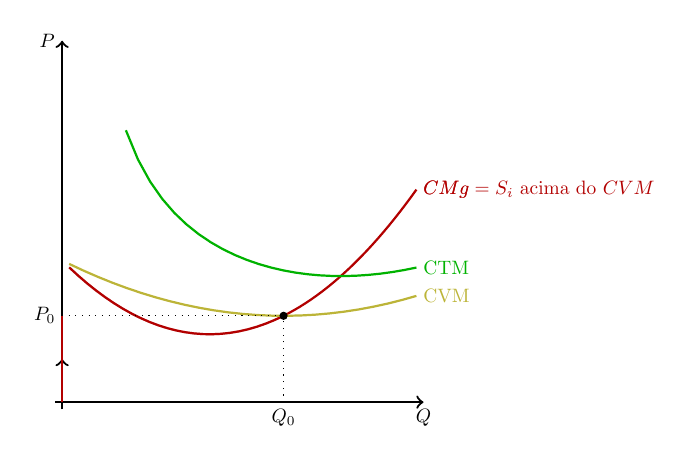
\begin{tikzpicture}[
			scale = 0.9,
			every node/.style = {scale =0.7},
			declare function = {
				cv(\x) = \x - (1/4)*\x^2 + (1/25)*\x^3;
				cf(\x) = 1;
				ct(\x) = cv(\x) + cf(\x);
				cmg(\x) = 1 - (2/4)*\x + (3/25)*\x^2;
				ctm(\x) = ct(\x)/\x;
				cvm(\x) = cv(\x)/\x;
			}
		]

			\def\p{3.9330669}
			\def\q{25/8}

			\draw[->,thick] (-0.1,-0) -- (5.1,-0) node[below]{$Q$};
			\draw[->,thick] (0,{cvm(\q)}) -- (0,5.1) node[left]{$P$};
			
			\onslide<1>{
				\draw[->,thick] (0,-0.1) -- (0,{cvm(\q)});
			}

			\draw[red!70!black,thick,domain=\q:5,variable=\x] plot (\x,{2*cmg(\x)-0});

			\onslide<1>{
				\draw[red!70!black,thick,domain=0.1:\q,variable=\x] plot (\x,{2*cmg(\x)-0});
			}

			\onslide<2->{
				\draw[red!70!black,opacity=0.3,thick,domain=0.1:\q,variable=\x] plot (\x,{2*cmg(\x)-0});
			}

			\onslide<1>{
				\draw[red!70!black](5,{2*cmg(5)-0})node[right]{$CMg$};	
			}

			\onslide<2->{
				\draw[red!70!black](5,{2*cmg(5)-0})node[right]{$CMg=S_i$ acima do $CVM$};
			}

			\draw[green!70!black,thick,domain=0.9:5,variable=\x] plot (\x,{2*ctm(\x)-0});	
		 	\draw[green!70!black](5,{2*ctm(5)-0})node[right]{CTM};
			 
			\draw[yellow!70!black,thick,domain=0.1:5,variable=\x] plot (\x,{2*cvm(\x)-0});
			\draw[yellow!70!black](5,{2*cvm(5)-0})node[right]{CVM};

			\onslide<2->{
				\draw[dotted] (0,{2*cmg(\q)})node[left]{$P_0$} -- (\q,{2*cmg(\q)});
				\draw[dotted] (\q,0)node[below]{$Q_0$}--(\q,{2*cmg(\q)})node[circle,fill,inner sep=1.5pt]{};
				\draw[thick,red!70!black] (0,0) -- (0,{2*cvm(\q)});
			}

		\end{tikzpicture}
	\end{center}
\end{frame}

\begin{frame}
	\frametitle{Curva da oferta}
	\'E o conjunto de pares $(Q,P)$ que constituem a escolha \'optima de uma empresa, considerando fixos todos os factores ex\'ogenos \`a decis\~ao da empresa:

	\vspace{0.5cm}

	pre\c cos dos inputs, tecnologia,...
\end{frame}

\begin{frame}
	\frametitle{Lei da Oferta}
	Entre a quantidade oferecida de um bem e o pre\c co desse mesmo bem, existe uma rela\c c\~ao positiva: se o pre\c co aumenta, a quantidade oferecida aumenta, \emph{c\ae teris paribus}.
\end{frame}

\begin{frame}
	\frametitle{Lei da Oferta}
	A Lei da Oferta adv\'em de:

	\vspace{0.4cm}

		Custos marginais de produ\c c\~ao crescentes, consequ\^encia de rendimentos marginais decrescentes na produ\c c\~ao --- para produzir mais uma unidade o custo adicional \'e cada vez maior, logo o pre\c co que os produtores est\~ao dispostos a receber tem de aumentar com a quantidade.

\end{frame}

\begin{frame}
	\frametitle{Oferta}
	\begin{columns}
		\begin{column}{0.65\textwidth}
			\begin{center}
				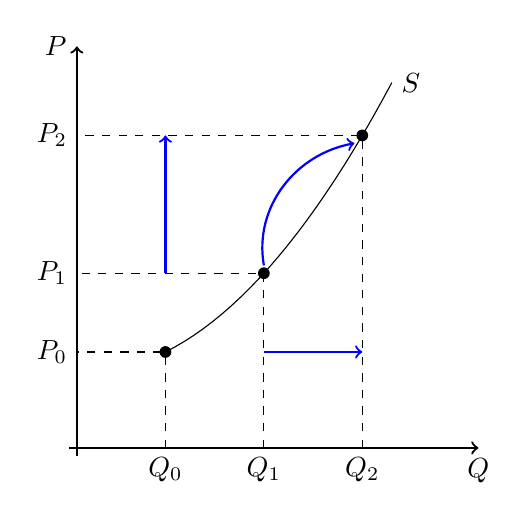
\begin{tikzpicture}[
					scale = 1,
					every node/.style = {scale =1},
					declare function = {
						s(\x) =  2*(1 - (2/4)*(\x+2) + (3/25)*(\x+2)^2); % > 25/8
					}
					]

				\def\q{25/8}
				\def\p{35/8}
				\def\r{45/8}

				\draw[->,thick] (-0.1,-0) -- (5.1,-0) node[below]{$Q$};
				\draw[->,thick] (0,-0.1) -- (0,5.1) node[left]{$P$};

				\draw[domain=(\q-2):4,variable=\x] plot (\x,{s(\x)});
				\draw(4,{s(4)}) node[right]{$S$};

				\draw[dashed]({\q-2},0)node[below]{$Q_0$} -- ({\q-2},{s(\q-2)})node[circle,fill,inner sep=1.5]{} -- (0,{s(\q-2)})node[left]{$P_0$};

				\onslide<2->{
					\draw[dashed]({\p-2},0)node[below]{$Q_1$} -- ({\p-2},{s(\p-2)})node[circle,fill,inner sep=1.5]{} -- (0,{s(\p-2)})node[left]{$P_1$};
				}

				\onslide<3->{
					\draw[dashed]({\r-2},0)node[below]{$Q_2$} -- ({\r-2},{s(\r-2)})node[circle,fill,inner sep=1.5]{} -- (0,{s(\r-2)})node[left]{$P_2$};
				}

				\onslide<4->{
					\draw[blue,thick,->] ({\q-2},{s(\p-2)}) -- ({\q-2},{s(\r-2)});
				}
				\onslide<5->{
					\draw[blue,thick,->] ({\p-2},{s(\q-2)}) -- ({\r-2},{s(\q-2)});
				}
				\onslide<6->{
					\draw[blue,thick,->] ({\p-2},{s(\p-2)+0.1}) to [out=100,in=190] ({\r-2-0.1},{s(\r-2)-0.1});
				}

				\end{tikzpicture}
			\end{center}
		\end{column}
		\begin{column}{0.3\textwidth}
			A Lei da Oferta descreve um movimento ao longo da curva:
			
			\vspace{0.5cm}

			A subida de pre\c co faz aumentar a quantidade oferecida, \emph{c\ae teris paribus}
		\end{column}
	\end{columns}
\end{frame}

\begin{frame}
	\frametitle{Inten\c c\~oes de Venda - Oferta}
	A quantidade de um bem que um produtor est\'a disposto a vender depende de:
	\begin{columns}
		\begin{column}{0.65\textwidth}
			\begin{itemize}
				\item \(p =\) pre\c co de venda {\color{red}(+)}
				\vspace{1cm}
				\item \(A =\) tecnologia de produ\c c\~ao{\color{red}(+)}
				\item \(r\ e\ w=\) pre\c co dos factores produtivos ($K$ e $L$){\color{red}(-)}
				\item $p_m$ = pre\c co de mat\'erias-primas{\color{red}(-)}
				\item $p_i$ = pre\c co de bens de consumo interm\'edio{\color{red}(-)}
				\item meteorologia (para o caso dos bens agr\'icolas){\color{red}(+)}
			\end{itemize}
		\end{column}
		\begin{column}{0.3\textwidth}
			\onslide<2->{
			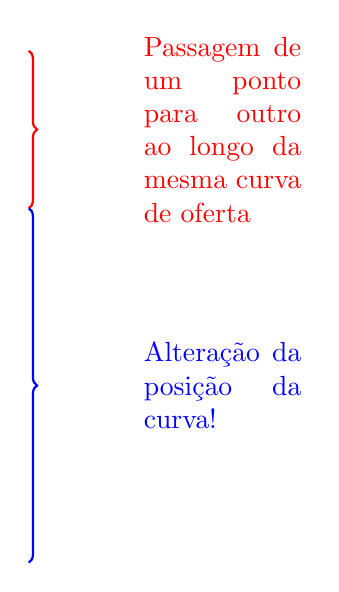
\begin{tikzpicture}[
				scale = 1,
				every node/.style = {scale = 1}
				]
				\draw [decorate,decoration={brace,mirror,amplitude=3pt},thick,red] (0,3) -- (0,5) node [midway,xshift=70pt] {\parbox{2cm}{Passagem de um ponto para outro ao longo da mesma curva de oferta}};
				
				\draw [decorate,decoration={brace,mirror,amplitude=3pt},thick,blue] (0,-1.5) -- (0,3) node [midway,xshift=70pt] {\parbox{2cm}{Altera\c c\~ao da posi\c c\~ao da curva!}};
			\end{tikzpicture}
			}
		\end{column}
	\end{columns}

\end{frame}

\begin{frame}
	\frametitle{Determinantes da Oferta}
	\begin{itemize}
		\item As vari\'aveis que levam \'a altera\c c\~ao da curva da oferta s\~ao ex\'ogenas \`a escolha da empresa e fazem com que as curvas de custo ou as curvas de produto se alterem.
		\item Havendo altera\c c\~ao das curvas de custo, h\'a altera\c c\~ao da curva da oferta.
		\item Uma altera\c c\~ao de pre\c co da venda, \emph{c\ae teris paribus} n\~ao faz alterar a curva da oferta, mas apenas se passa de um ponto na mesma curva.
	\end{itemize}
\end{frame}

\begin{frame}
	\frametitle{Oferta}
	\begin{itemize}
		\item \`A rela\c c\~ao funcional entre a quantidade oferecida de um bem e todas as vari\'aveis que a influenciam, chama-se \underline{Fun\c c\~ao Oferta:}\[Q_s=f(p,r,w,A,p_i,p_m,...)\]
		\item A curva de oferta obt\'em-se, estudando a rela\c c\~ao que existe entre a quantidade oferecida $Q_s$ e $p$, para valores dados das outras vari\'aveis (ex\'ogenas)
	\end{itemize}
	Diferentes valores das vari\'aveis ex\'ogenas geram curvas de oferta diferentes --- movimenta\c c\~ao da oferta no espa\c co ($Q,P$)
\end{frame}

\begin{frame}
	\frametitle{Expans\~ao da Oferta}
	\begin{center}
		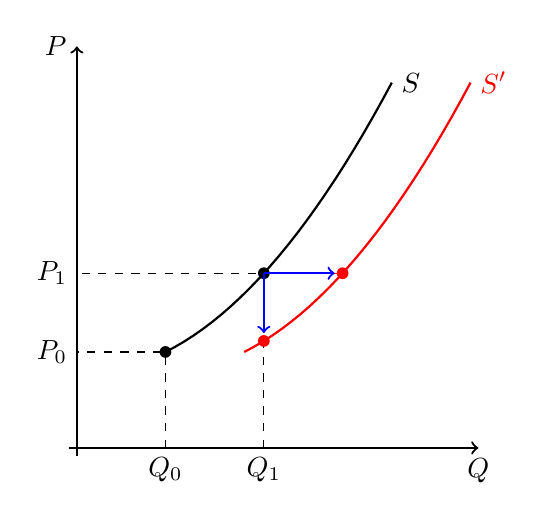
\begin{tikzpicture}[
			scale = 1,
			every node/.style = {scale =1},
			declare function = {
				s(\x) =  2*(1 - (2/4)*(\x+2) + (3/25)*(\x+2)^2); % > 25/8
			}
			]

		\def\q{25/8}
		\def\p{35/8}
		\def\r{45/8}

		\draw[->,thick] (-0.1,-0) -- (5.1,-0) node[below]{$Q$};
		\draw[->,thick] (0,-0.1) -- (0,5.1) node[left]{$P$};

		\draw[thick,domain=(\q-2):4,variable=\x] plot (\x,{s(\x)});
		\draw({5-1},{s(5-1)}) node[right]{$S$};

		\draw[dashed]({\q-2},0)node[below]{$Q_0$} -- ({\q-2},{s(\q-2)})node[circle,fill,inner sep=1.5]{} -- (0,{s(\q-2)})node[left]{$P_0$};

		\onslide<2->{
			\draw[thick,red,domain=(\q-1):5,variable=\x] plot (\x,{s(\x-1)});
			\draw[red](5,{s(5-1)}) node[right]{$S'$};
			\draw[dashed]({\p-2},0)node[below]{$Q_1$} -- ({\p-2},{s(\p-2)})node[circle,fill,inner sep=1.5]{} -- (0,{s(\p-2)})node[left]{$P_1$};
		}

		\onslide<3->{
			\draw[dashed,red]({\p-2},{s(\p-2)}) -- ({\p-1},{s(\p-2)})node[circle,fill,inner sep=1.5]{};

			\draw[red] ({\p-2},{s(\p-3)}) node[circle,fill,inner sep=1.5]{};

			\draw[blue,thick,->] ({\p-2},{s(\p-2)}) -- ({\p-1-0.1},{s(\p-2)});
			\draw[blue,thick,->] ({\p-2},{s(\p-2)}) -- ({\p-2},{s(\p-3)+0.1});
		}

		\end{tikzpicture}
	\end{center}
	\onslide<4->{Que altera\c c\~ao de vari\'aveis ex\'ogenas poderia estar na origem da desloca\c c\~ao da oferta?}
\end{frame}

\begin{frame}
	\frametitle{Expans\~ao da Oferta}
	\begin{center}
		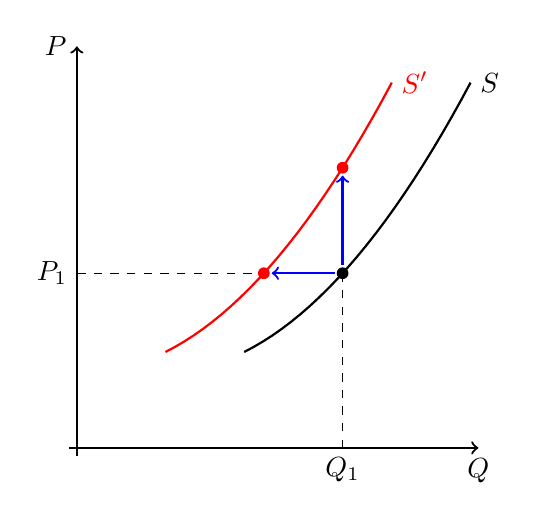
\begin{tikzpicture}[
			scale = 1,
			every node/.style = {scale =1},
			declare function = {
				s(\x) =  2*(1 - (2/4)*(\x+2) + (3/25)*(\x+2)^2); % > 25/8
			}
			]

		\def\q{25/8}
		\def\p{35/8}
		\def\r{45/8}

		\draw[->,thick] (-0.1,-0) -- (5.1,-0) node[below]{$Q$};
		\draw[->,thick] (0,-0.1) -- (0,5.1) node[left]{$P$};

		\draw[thick,domain=(\q-1):5,variable=\x] plot (\x,{s(\x-1)});
		\draw(5,{s(5-1)}) node[right]{$S$};

		\onslide<2->{
			\draw[thick,red,domain=(\q-2):4,variable=\x] plot (\x,{s(\x)});
			\draw[red]({5-1},{s(5-1)}) node[right]{$S'$};
		}

		\onslide<3->{
			\draw[dashed]({\p-1},0)node[below]{$Q_1$} -- ({\p-1},{s(\p-2)})node[circle,fill,inner sep=1.5]{} -- (0,{s(\p-2)})node[left]{$P_1$};
		}

		\onslide<4->{

			\draw[red] ({\p-2},{s(\p-2)})node[red,circle,fill,inner sep=1.5]{};
			\draw[red] ({\p-1},{s(\p-1)})node[red,circle,fill,inner sep=1.5]{};

			\draw[blue,thick,->] ({\p-1-0.1},{s(\p-2)}) -- ({\p-2+0.1},{s(\p-2)});
			\draw[blue,thick,->] ({\p-1},{s(\p-2)+0.1}) -- ({\p-1},{s(\p-1)-0.1});
		}

		\end{tikzpicture}
	\end{center}
	\onslide<4->{Que altera\c c\~ao de vari\'aveis ex\'ogenas poderia estar na origem da desloca\c c\~ao da oferta?}
\end{frame}

\begin{frame}
	\frametitle{Oferta}
	\begin{center}
		No mercado de concorr\^encia perfeita, a curva da oferta de uma empresa \'e a curva de custos marginais acima do limiar de encerramento.

		\vspace{1cm}

		A oferta de mercado resulta da adi\c c\~ao de todas as ofertas individuais
	\end{center}
\end{frame}

\begin{frame}
	\frametitle{Modelos lineares para a Oferta}
		Para simplifica\c c\~ao de c\'alculo, \'e frequente utilizar-se modelos lineares para a oferta, na forma:
		\[Q=c+d\times P \quad \text{(forma directa)}\] ou \[P=-\frac{c}{d}+\frac{1}{d}\times Q\text\quad\text{(forma inversa)}\]
		Seja qual for a forma, representa-se sempre no espa\c co $(Q,P)$, devido a Marshall (1895) ``Principles of Economics''
\end{frame}

\begin{frame}
	\frametitle{Modelos Lineares para a Oferta: interpreta\c c\~oes}
	\begin{columns}
		\begin{column}{0.6\textwidth}
			\begin{center}
				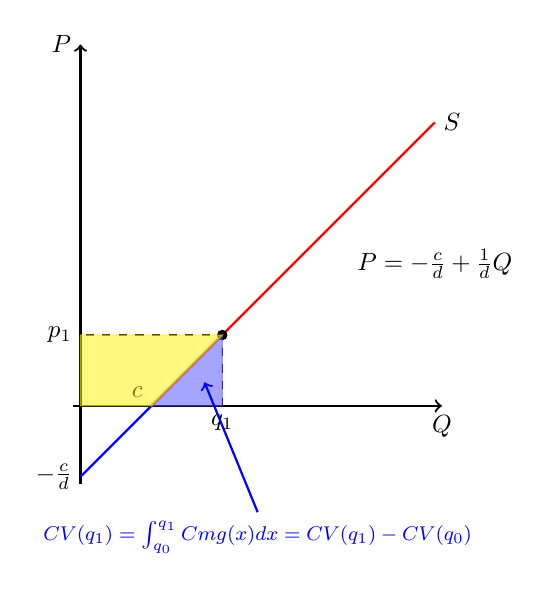
\begin{tikzpicture}[
					scale = .9,
					every node/.style = {scale = .9},
					declare function = {
						s(\x) = -(1/1)+(1/1)*\x;
					}]

					\draw[->,thick] (-0.1,-0) -- (5.1,-0) node[below]{$Q$};
					\draw[->,thick] (0,-1.1) -- (0,5.1) node[left]{$P$};

					\draw[blue,thick,domain=0:1,variable=\x] plot (\x,{s(\x)});
					\draw[red,thick,domain=1:5,variable=\x] plot (\x,{s(\x)});
					
					\draw(0,{s(0)}) node[left]{\(-\frac{c}{d}\)};
					\draw(1,{s(1)}) node[above left] {$c$};

					\draw(5,{s(5)}) node[right]{$S$};

					\draw(5,{s(5)/2}) node[]{\(P=-\frac{c}{d}+\frac{1}{d}Q\)};

					\draw[dashed](2,0) node[below]{$q_1$} -- (2,{s(2)})node[circle,fill,inner sep=1.5]{} -- (0,{s(2)})node[left]{$p_1$};

					\onslide<2->{
						\draw[fill,blue!70!white,opacity=0.5] (1,0) -- (2,0) -- (2,{s(2)}) -- (1,0);
						\draw[<-,blue,thick] (1.75,{s(2)/3}) -- (2.5,{-s(2)-0.5})node[below]{\footnotesize\(CV(q_1)=\int^{q_1}_{q_0}Cmg(x)dx=CV(q_1)-CV(q_0)\)};
					}

					\onslide<3->{
						\draw[fill,yellow,opacity=0.5] (0,0) -- (1,0) -- (2,{s(2)}) -- (0,{s(2)}) -- (0,0);
					}

				\end{tikzpicture}
			\end{center}
		\end{column}
		\begin{column}{0.4\textwidth}
			{
			\small
			\begin{itemize}
				\item Para produzir $q_1$, no minimo os produtores t\^em de receber $p_1$ por unidade, ou, ao pre\c co $p_1$ o m\'aximo que os produtores est\~ao dispostos a produzir \'e $q_1$
				\item $p_1\times q_1$ \'e a receita de vendas; a \'area do triangulo abaixo da Oferta at\'e $q_1$ s\~ao os custos vari\'aveis... a diferen\c ca entre receita e custos vari\'aveis \'e o {\colorbox{yellow}{\textbf{Excedente de Produtor!}}}
			\end{itemize}
			\normalsize
			}
		\end{column}
	\end{columns}
\end{frame}

\begin{frame}
	\frametitle{Excedente do Produtor}
	Por unidade do bem transaccionado, \'e a diferen\c ca entre o que o produtor recebe por unidade e o m\'inimo que estaria disposto a receber para produzir e fornecer essa unidade (valor dado pela curva de oferta)
	
	\vspace{0.5cm}

	O excedente total do produtor \'e o somat\'orio dos excedentes individuais de cada produtor e corresponde graficamente \`a \'area acima da curva de oferta at\'e ao pre\c co.

	\vspace{0.5cm}

	Para empresas economicamente vi\'aveis, o excedente \'e necessariamente n\~ao negativo, o que pode consistir em lucro ou preju\'izo a curto prazo, consoante o n\'ivel de custos fixos.
\end{frame}

\begin{frame}
	\frametitle{Excedente do Produtor}

	\[\text{Lucro}=RT-CV-CF\] 

	\vspace{1cm}

	\[\text{Lucro} = \text{Excedente de produtor} - CF\]

	\vspace{1cm}

	Exerc\'icios recomendados: Caderno 3 $\rightarrow$ 8, 9, 10 e 12.
\end{frame}